% Fig. — Note to linked chart. Full-width spine; shared workflow type scale.
\documentclass[tikz,border=1.5pt]{standalone}
\usepackage[T1]{fontenc}
\usepackage{lmodern}
\usepackage{helvet}
\renewcommand{\familydefault}{\sfdefault}
\usepackage{tikz}
\usetikzlibrary{arrows.meta,calc}

\definecolor{llmfill}{HTML}{334155}
\definecolor{llmbord}{HTML}{1E293B}
\definecolor{codefill}{HTML}{E2E8F0}
\definecolor{codebord}{HTML}{64748B}
\definecolor{cardbg}{HTML}{FFFFFF}
\definecolor{ink}{HTML}{0F172A}

% Shared workflow typography (Helvetica)
\newcommand{\wffont}{\sffamily\fontsize{7.75}{9.0}\selectfont}
\newcommand{\wfleg}{\sffamily\fontsize{7.25}{8.25}\selectfont\bfseries}

\begin{document}
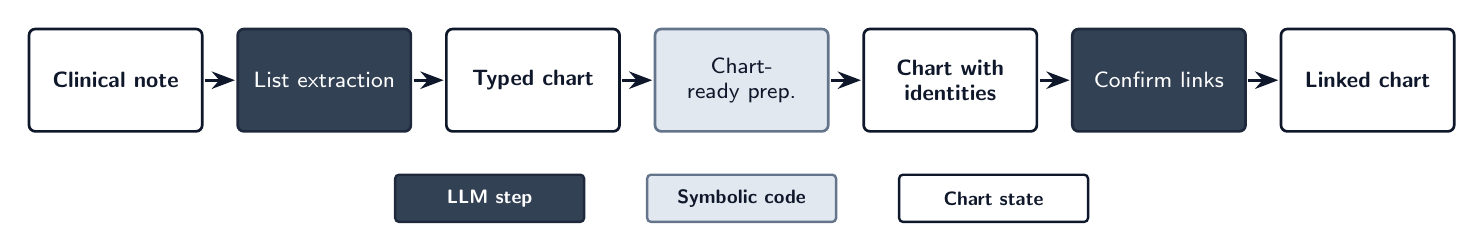
\begin{tikzpicture}[x=1mm,y=1mm,>=Stealth,font=\wffont,text=ink,
  every node/.style={align=center}]
  \tikzset{
    stepnode/.style={
      draw, line width=0.34mm, rounded corners=0.8mm, align=center,
      minimum width=22mm, minimum height=13mm,
      text width=20mm, inner sep=0.5mm,
      font=\wffont
    },
    model/.style={stepnode, draw=llmbord, fill=llmfill, text=white},
    code/.style={stepnode, draw=codebord, fill=codefill, text=ink},
    state/.style={stepnode, draw=ink, fill=cardbg, text=ink, font=\wffont\bfseries},
    arr/.style={->, line width=0.42mm, draw=ink, shorten >=0.5pt, shorten <=0.5pt},
    leg/.style={
      draw, line width=0.30mm, rounded corners=0.5mm, align=center,
      minimum width=24mm, minimum height=6mm, inner sep=0.4mm,
      font=\wfleg
    }
  }

  % Full-width row: centers 11 .. 170 (pitch 26.5), content center 90.5
  \node[state] (n0) at (11,0) {Clinical note};
  \node[model] (n1) at (37.5,0) {List extraction};
  \node[state] (n2) at (64,0) {Typed chart};
  \node[code] (n3) at (90.5,0) {Chart-ready prep.};
  \node[state] (n4) at (117,0) {Chart with\\identities};
  \node[model] (n5) at (143.5,0) {Confirm links};
  \node[state] (n6) at (170,0) {Linked chart};

  \foreach \a/\b in {n0/n1,n1/n2,n2/n3,n3/n4,n4/n5,n5/n6}
    \draw[arr] (\a) -- (\b);

  % Legend centered on content center 90.5 (pitch 32)
  \node[leg, draw=llmbord, fill=llmfill, text=white] at (58.5,-15) {LLM step};
  \node[leg, draw=codebord, fill=codefill, text=ink] at (90.5,-15) {Symbolic code};
  \node[leg, draw=ink, fill=cardbg, text=ink] at (122.5,-15) {Chart state};
\end{tikzpicture}
\end{document}
